\documentclass{article}
\usepackage{graphicx}
\usepackage{subfig}
\usepackage{float}
\usepackage{amssymb}% http://ctan.org/pkg/amssymb
\usepackage{pifont}% http://ctan.org/pkg/pifont
\newcommand{\cmark}{\ding{51}}%
\newcommand{\xmark}{\ding{55}}%

\graphicspath{ {images/} }
\begin{document}

\section{Introduction}
Range searching problems are common in computational geometry. Finding the number of points inside a polygon and its attributes find its application in areas that deal with processing geometrical data, such as computer graphics, computer vision, geographical information systems (GIS), motion planning, and CAD. 

There has been a significant amount of successful work done using GPUs on regular applications that have more structured access to memory and have  large amount of data parallelism so that it be efficiently implemented on a SIMD model.However the GPU implementation of irregular algorithms such as traversal of a pointer based quadtree is challenging as the traversal of a point is input data dependent and running multiple traversals simultaneously leads to thread divergence and unpredictable memory access.In this paper we investigate GPU traversal of a pointer based quadtree data structure built on the CPU.And instead of querying individual points, we query the points inside a region which are assumed to be regular polygons.
Implementation of quadtree/octree traversal on CUDA GPU either uses DFS or BFS algorithms. 
The paper "A sparse octree gravitational N-body code that runs entirely on the GPU processor",ignores DFS and implements  BFS as only the latter can be vectorized and it implements stack based BFS traversal to achieve parallelism.

GPU CUDA ray traversal through a hierarchical data structure such as a bounding volume hierarchy (BVH) is usually carried out using depth-first search  by maintaining a stack.
But rather than parallelizing the search for a single ray, many rays are run simultaneously.
To accelerate this DFS search algorithm on GPUs another option would be to begin the search few layers deep in the tree, where there are as many intermediate nodes as parallel threads. Then each thread starts its own depth-first search.

This paper investigates the efficient ways to perform a range-searching problem.
The first approach is the traditional brute force search method.This method is implemented on the CPU as well as the GPU. In the CPU implementation, all input points are checked  sequentially to see if they lie within the query polygon boundary. In the GPU implementation, all the input points are checked simultaneously by assigning each point to a thread. Each thread checks the point against all the query polygons and returns the attributes of all the polygons that contain the point. If the number is threads launched is lesser than the input points, then the threads loop over to take the next set of points.
The second method uses a pointer based quadtree data structure to find the points inside the regular polygon on the CPU. In the CPU approach, to traverse the tree, a recursive Depth first search algorithm is implemented.
In the third method, the algorithm to find the points inside the polygon is implemented on the GPU  using the quadtree built on the CPU.In this approach, traversing a pointer based quadtree data structure using stack based BFS has been implemented to find the points inside a regular polygon region.In order to accelerate the traversal, BFS starts at level 3 of the quadtree.

Range search algorithms, which make use of spatial data structures, perform much better than the ones that do not partition the data before processing. Quadtree is a hierarchical spatial data structure that is used for both indexing and compressing geographic database layers due its applicability to many types of data,its ease of implementation and relatively good performance. The point quadtree structure recursively divides space into equal four rectangles based on the location of the points. The root of the quadtree represents the whole 2D space. Successive points divide each new sub-region into quadrants until all points are indexed.

As done traditionally, the quadtree is built on the CPU. To speed up the range searching problems, it is essential to increase the threshold on the number of queries processed within a given time frame.Purely sequential approach to this will demand increase in processor speeds.And growth in processor speed on a single core has reached its threshold due to the properties of silicon because of  the increase in power consumption.Therefore parallel computing is the only solution to increase the threshold on the number of inputs processed. 
We use NVIDIAs CUDA programming model for the GPU, which allows us to execute thousands of threads simultaneously on the GPU. In CUDA, the CPU executes the sequential part of the code and the computationally intensive part, which has more scope for parallelization, is done in the GPU. 

In this paper we prove that the CPU-GPU approach shows a performance improvement by a factor of 4x to 500x compared to the pure CPU approach.





\section{Motivation and Background}

In theory ,for n items, the quadtree gives a  performance of ${(n*log(n))}$ .Compared to a brute force method's performance of $n^{(2)}$ , a quadtree is extremely fast. So the performance gain by using a quadtree is ${(log(n))/n}$.  
As shown in Fig 1, the empirical investigation of quadtree search and brute force search shows that the quadtree has a 9x better performance for medium number of queries and 8x improvement for larger problems.
The main purpose of quadtree lies in localizing the queries.The brute force search on a CPU checks sequentially if every single point of the input data satisfies the criteria whereas quadtrees help isolate the region of interest faster by ignoring the quadrants of the tree that lie outside the region of interest at every level, thus reducing the number of quadrants to be processed at the next level.Therefore the quadtree gives better performance for a dense more concentrated data than a dense equally distributed data set.


\begin{figure}[H]
\centering
    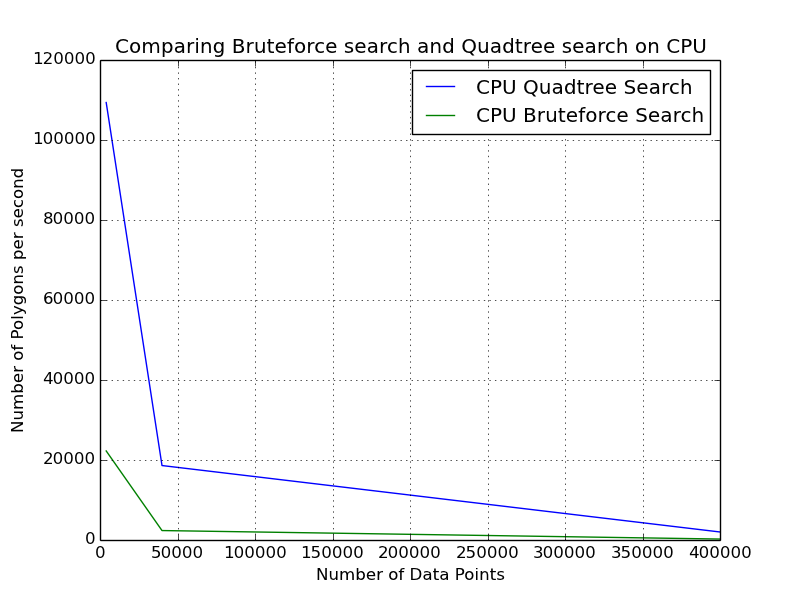
\includegraphics[scale=0.55]{BruteVsQuadCPU_logscale_new_2}
    \caption{Comparing Bruteforce search and Quadtree search on CPU}
  \end{figure}

\begin{figure}[H]
\centering
    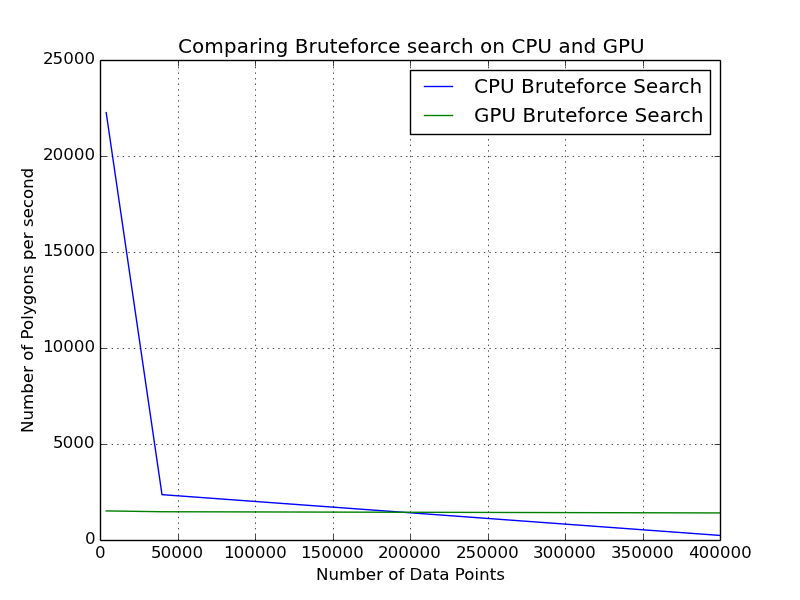
\includegraphics[scale=0.55]{CPU_GPU_brute_new_2}
    \caption{Comparing Bruteforce search on CPU with GPU}
  \end{figure}



As shown in Fig 2, the GPU provides a better performance for brute force search compared to CPU for larger datasets.But this performance is still lower than the CPU performance using a Quadtree.
The same algorithm is used for both CPU and GPU brute force search to check if a point is within the Polygon. But the  GPU is capable of launching 65535 blocks with a maximum of 1024 threads, thus massively parallelizing the search.
The Geforce GTX680 Kepler architecture used, has a new parallel geometry pipeline optimized for tessellation and displacement mapping.And also it has a better performance /watt.

This paper investigates the performance improvement of the GPU implementation of points inside a polygon search using a Quadtree .


\begin{figure}[H]
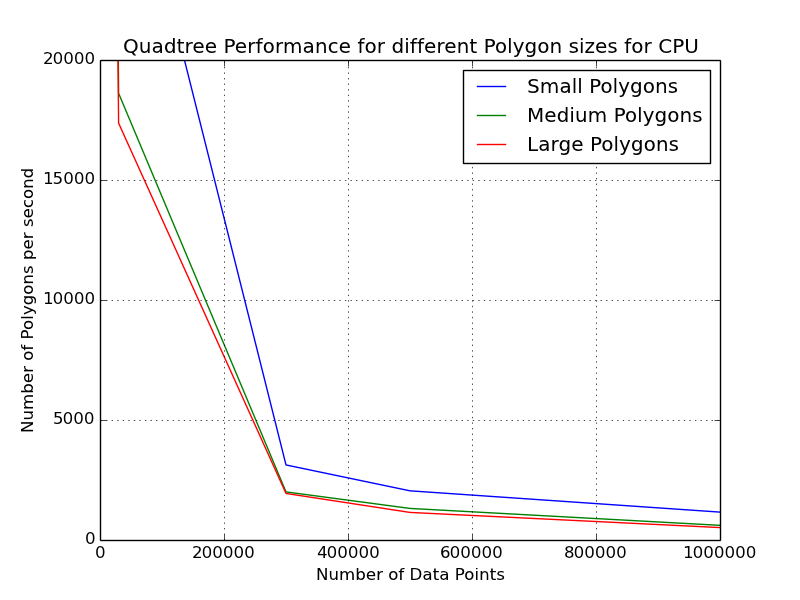
\includegraphics[scale=0.6]{Different_Sized_Polygon_logScale_cpu04_10}
\caption{Performance analysis on Quadtree CPU using Polygons of different sizes}
\end{figure}

The Fig 3 shows the quadtree performance for different sized polygons.It  performs better on small polygons compared to larger polygons.The performance improvement in this case relates to how quickly the quadrants of the quadtree that contain the polygon can be isolated.The amount of computation done for a larger polygon that occupies all four quadrants is higher compared to a smaller polygon that lies inside only one quadrant.



\subsection{GPU Architecture}

 \begin{figure}[H]
 \centering
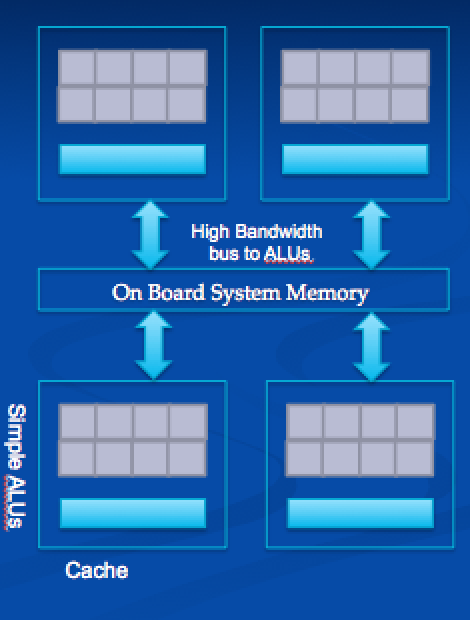
\includegraphics[scale=0.8]{GPU_Architecture}
\caption{Modern GPU Architecture}
 \end{figure}
 
 

For range searching problem,the GPUs are better compared to CPUs due to their highly data-parallel nature and the ability to achieve higher arithmetic intensity.Both floating point operations per second (FLOPS) and chip bandwidth continue to increase at much faster rate on the GPU compared to CPU.
 
 
 Another significant factor is that the GPU computation is more power and cost efficient than the CPU.
This performance gap is due to the difference in the design of CPU and GPU. 
CPUs are designed as latency oriented cores.It has powerful ALU units to reduce operational latency,large cache to reduce memory access latency and sophisticated control logic to reduce branch  prediction latency and data forwarding latency(the latency between the generation of data value and the execution of all instructions that require the data as input). On the other hand, the GPUs are designed as throughput oriented cores which exploits  data parallelism to achieve higher throughput. In order to increase throughput ,it has smaller caches , less sophisticated control logic with no branch prediction and very little data forwarding, and very large number of low power ALUs that are heavily pipelined.Thus it dedicates more of its chip area to ALU units rather than cache or control logic.Massive number of threads are required in order to utilize the throughput nature of the GPU and to overcome the long operational latencies. Due to these reasons GPUs perform better than CPU for larger datasets when maximum number of threads are launched whereas the performance is lower, sometimes even lesser than the CPU for smaller datasets when very less number of threads are active.
 
 
GPU implements a Single instruction multiple data (SIMD) model unlike the traditional CPU architectures where each thread may execute its own set of instructions. Multiple processing units are controlled by the same control signal from the control unit. Though each unit executes the same instruction, they have different data that corresponds to the CUDA threads.
 
For the GPU implementation of the problem, we focus on NVIDIA 's Geforce GTX 680 architecture and the CUDA programming language. This generation of the CUDA enabled GPU devices consists of an array of 8 next generation streaming multiprocessors (SMX) , 4 GPC and 4 memory controllers.Each GPC has a dedicated raster engine and two SMX units. The eight SMX units are massively threaded and are capable of executing hundreds of threads in parallel.Each SM contains a set of simple cores called streaming processors, or SPs, which are responsible for executing an instruction for a single thread.And these SPs of a single SMX share the same control logic and instruction cache and therefore execute the same instruction but with different data input.

 \begin{figure}[H]
 \centering
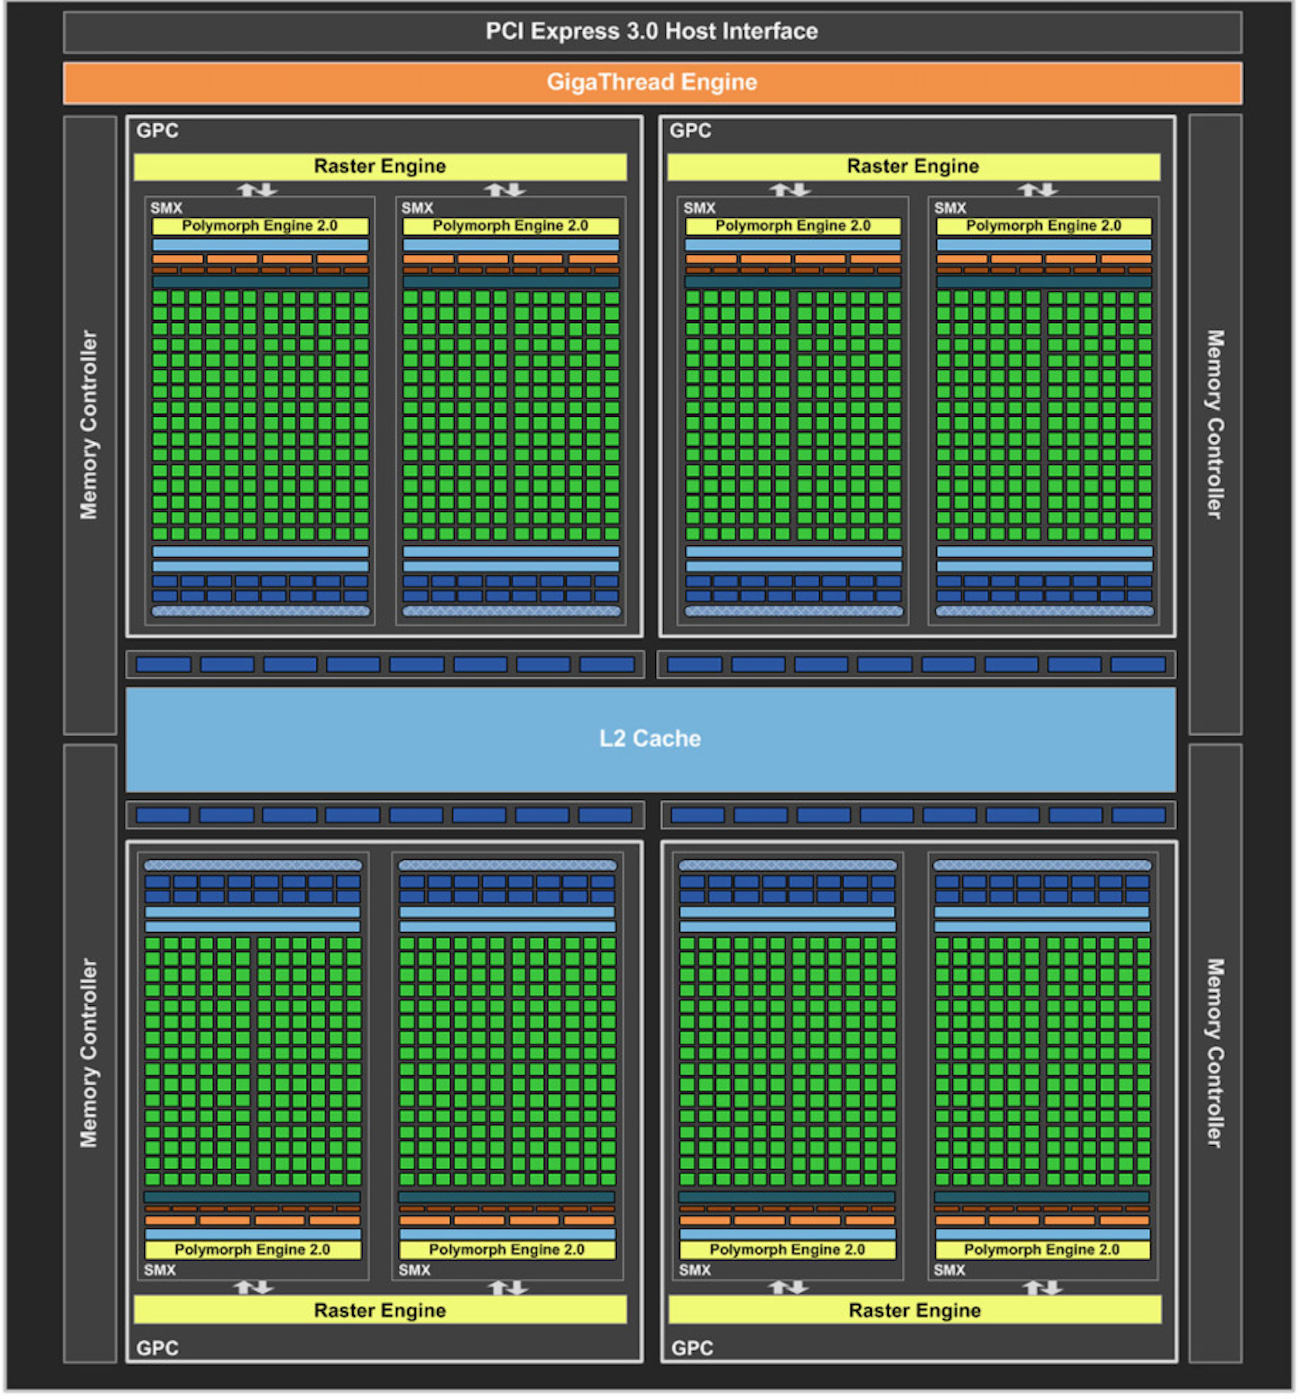
\includegraphics[scale=0.5]{KeplerArch}
\caption{Kepler Architecture}
 \end{figure}

Languages like Brook, CUDA and OpenCL , Harlan allow the GPU to be used efficiently for non-graphics related problems.We use NVIDIA's CUDA programming model for the GPU,a heterogeneous parallel  programming model that enables exploitation of data parallelism by using both CPU and GPU.It allows us to execute thousands of threads simultaneously on the graphics processing unit (GPU). 
CUDA is developed as an extension to C/C++ programming languages.The sequential portion of the problem is assigned to the CPU and the CPU invokes a kernel code assigning the parallel portion of the problem to the GPU.The developer decides the size of data assigned to a block and the number of threads within each block that needs to be launched to process the data.The GPU hardware maps the data blocks to the SMX through time and space multiplexing.
Since each SMX has limited hardware resources such as shared memory, registers , number of threads that can be tracked and scheduled (scheduling slots ), careful selection of block sizes allows the SMX to accommodate more blocks simultaneously thus increasing the throughput.
SMX schedules thread execution and threads are assigned to SMX in block granularity. In the current generation of CUDA, we can assign up to 8 blocks to each SMX.With a total of eight SMX units, the GeForce GTX 680 implementation has 1536 CUDA Cores.
Threads running in an SM are scheduled in groups of 32, called a warp, and execute in SIMD fashion on a set of SPs. Warps are further grouped into large blocks of threads. Warps performing long running operations such as global memory accesses yield to allow other warps to proceed with execution to overcome latency.
Each SMX unit contains four warp schedulers, and each warp scheduler is capable of dispatching two instructions per warp every clock.
One feature of CUDA which reduces the software engineering effort is its transparent scalability. This means that the CUDA  kernel can be scaled to any number of processors.

The CUDA memory model consists of a global memory which is the GDDR DRAM , shared memory , and registers.Shared memory is a software controlled cache that is present in the SMX and all the processing units within the SM have access to the same shared memory.And all the SMX have access to the global memory on the device.Shared memory has lower latency and higher throughput accessibility compared to global memory.Global memory is capable of achieving much higher throughput if the threads from a warp access data from multiple consecutive locations rather than random locations.In this case, the hardware coalesces, all of these accesses into a consolidated access to consecutive DRAM locations.



\clearpage
\section{Implementation}

\subsection{Quadtree Construction}

Figure 6 to Figure 9 demonstrates quadtree construction on the CPU up to level 4.

A quadtree is a tree data structure in which each internal node has exactly four children. Quadtrees are most often used to partition a two-dimensional space by recursively subdividing it into four quadrants or regions. If a child node does not contain any data points, then that node is marked as null and it is not subdivided further.

 \begin{figure}[ht]
   \centering
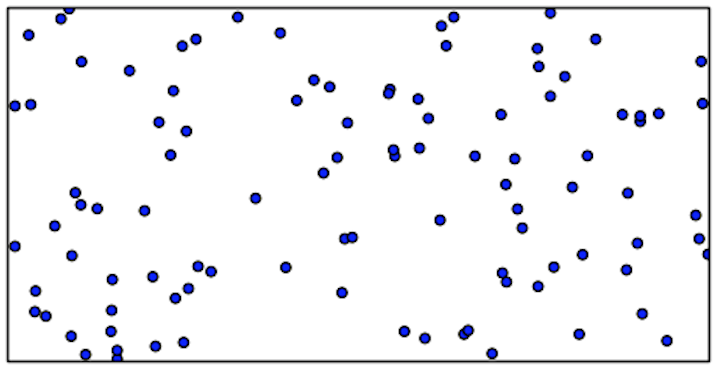
\includegraphics[scale=0.5]{Quadtree_construction1}
\caption{Level 1 of Quadtree}
 \end{figure}
 
  \begin{figure}[ht]
    \centering
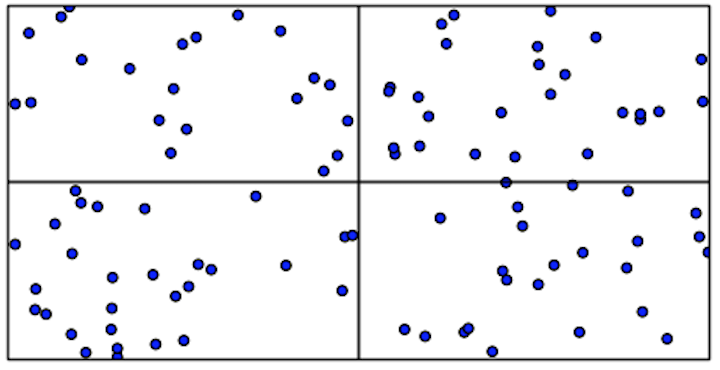
\includegraphics[scale=0.5]{Quadtree_construction2}
\caption{Level 2 of Quadtree}
 \end{figure}
 
  \begin{figure}[ht]
    \centering
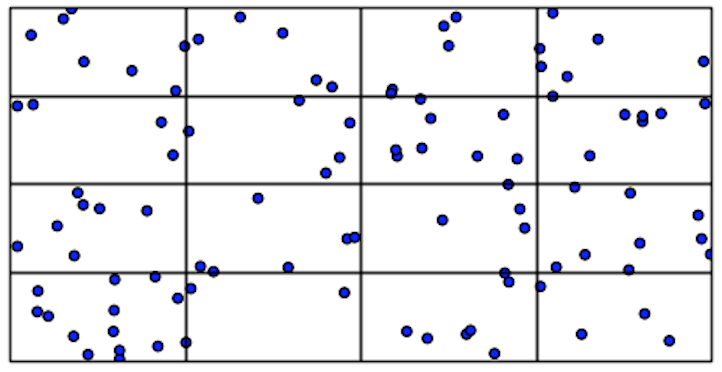
\includegraphics[scale=0.5]{Quadtree_construction3}
\caption{Level 3 of Quadtree}
 \end{figure}
 
  \begin{figure}[ht]
    \centering
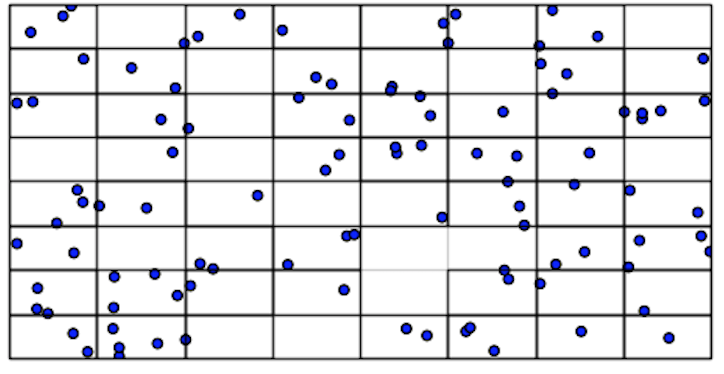
\includegraphics[scale=0.5]{Quadtree_construction4}
\caption{Level 4 of Quadtree}
 \end{figure}

\clearpage
The common algorithm to construct a quadtree is based on sequential point insertion and this sequential approach is not suitable for massively parallel processors.Therefore the quadtree construction is done on the CPU.
 The performance of quadtrees,  for Insertion is O(n log n) , for searching is O(log n) and optimization for the purposes of balancing the tree is O(nlogn). This makes quadtrees an ideal data structure for multiple insertion of points and range searching.
 Though the linear quadtrees reduce the overhead involved in transferring the tree from the CPU main memory to the GPU memory,the pointer based quadtree has several other advantages.
 The pointer based quadtrees are more memory space efficient.It can be accessed in any traversal order by  following the pointers whereas the linear quadtree only allows preorder traversal and require logarithm time searches to find the next child for any other order.
 
The Quadtree is built using pointers.The tree is built by recursive function calls and sequentially inserting the points. Each parent node has pointers to all of its children.There are 3 structures in the quadtree, the node, the point and the point buffers. 

The node is of 3 types which are the root node, link node and the leaf node.The root node,  corresponds to the entire array of input points.The four children of the root node represent the 4 quadrants (Northwest - NW, Northeast - NE,Southwest - SW,Southeast - SE).The link node is a node that can be further subdivided and the leaf nodes correspond to the quadrants for which further subdivision is not necessary. 

The point structure is the input points to the quadtree which occupies a 2D space. Each leaf node has a list of point buffers each of which holds pre-determined maximum number of points.

Starting at the root, the quadrant which the input point occupies is determined. We recurse down the tree to determine the direction(NW,NE,SW,SE) of the point until the leaf node is reached. 
Then,  the point is added to that leaf node's buffer of points. If the buffer exceeds some pre-determined maximum number of elements , the points are moved into the next buffer in the buffer list. 
The root node is subdivided recursively. The quadtree with k levels including the root would have ${(4(k-1))}$ nodes on the kth level and  ((4k) $-1$) nodes in total.


\subsection{CPU implementation}

The traversal starts from the root node of the quadtree and performs DFS by recursion.
It runs recursively till leaf node is reached.Depth First Search algorithm(DFS) traverses a graph in a depth wise motion and uses recursive function to get the next node to start a search when the bottom of the tree is reached.It starts at the root node and moves down the tree till the bottom of the tree is reached along each branch before backtracking.

While visiting each node,it checks for all three conditions to see if a node is completely overlapping, partially overlapping or not overlapping.



Table 1 illustrates the conditions to satisfy each scenario. N0,N1,N2 and N3 are the four corners of a node and the boundary of the polygon is marked by the four corners, P0, P1, P2, P3  of a rectangle. A checkmark indicates that the corners of the node is within the boundary of all four edges of a polygon. A x mark indicates that the corner of the node is outside the boundary of all four edges of a polygon.
If all the corners of a node is within the four edges of a polygon,then the node is completely overlapping the polygon.
If all the corners of a node is outside the four edges of a polygon,then the node is not overlapping the polygon.
If at least one of the corner of a node is outside the four edges of a polygon,then the node is Partially overlapping the polygon. All the conditions apart from the ones shown in Table 1 are partially overlapping.

\begin{table}[H]
\caption{Criteria for Quadtree node classification }
\centering
\begin{tabular}{c c c c c c}
\hline\hline
Case & N0 & N1 & N2 & N3 & Condition \\ [0.5ex] % inserts table 
%heading
\hline
P0 P1 P2 P3 & \checkmark & \checkmark & \checkmark & \checkmark & Completely overlapping \\
P0 P1 P2 P3 & \xmark & \xmark & \xmark & \xmark & Not overlapping \\

\hline
\end{tabular}
\label{table:nonlin}
\end{table}





Before classifying the node as not overlapping,we also check if the polygon is inside the node.
If the node is classified as completely overlapping node, then the boundary details of this node is stored and tree is not traversed further from this node.The boundary of the node represents the range of points the node contains and all these points within the node are considered as points within the polygon.
If the node is classified as not overlapping node, then the tree is not traversed further from this node.
If the node is classified as partially overlapping  node then the tree is traversed further till the leaf node is reached.The points are then extracted from the leaf nodes of the quadtree.

In the case of partially overlapping node, every point needs to be checked to see if it lies within the boundary of the polygon.This check is optimized by classifying the kind of intersection between the node  and the Polygon in such a way that for certain scenarios only either x or y coordinate of the points need to be verified.

\begin{figure}[H]
\caption{Different scenarios of overlap between node and polygon}
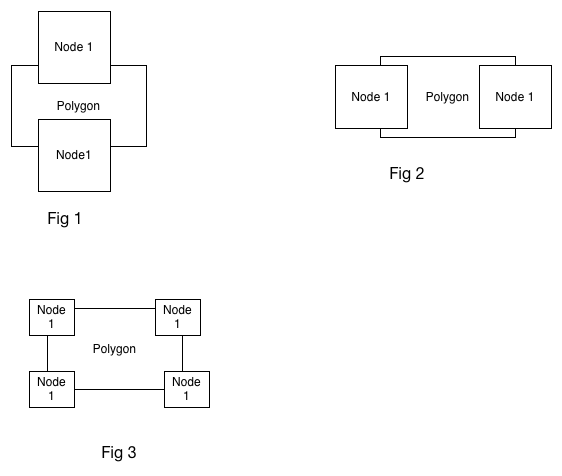
\includegraphics[scale=0.5]{OverlapScenario}
\end{figure}

If the intersection of the node is as in Fig1 ,then only the x co-ordinate of the point needs to be checked as all the y-coordinates of all points is within the polygon boundary limits.

If the intersection between the node and the polygon is as in Fig 2 ,then only the y co-ordinate of the point needs to be checked as all the x-coordinates of all points is within the polygon boundary limits.

For Fig 3 and all the other conditions, x-y co-ordinate of every point is checked against the boundary limits of the polygon.

In the case of GPU implementation, x-y coordinates of all points are checked against the polygon without classifying them based on the type of node intersection as it will lead to more conditional statements which would increase thread divergence and reduce the performance.



\subsection{GPU Implementation}

Efficient implementation of Quadtree traversal in GPU using CUDA is challenging due to the following reasons. 1. The Quadtree is an irregular data structure whose memory accesses and work distribution are both irregular and data-dependent and traversing irregular data structure results in thread divergence.
2.Traversal of a Quadtree built using pointers results in lot of pointer-chasing memory operations.Pointer-chasing leads to many uncoalesced memory accesses which affects performance. 
3. As done typically the Quadtree is built using recursive depth first style in the CPU. Recursive DFS in GPU would be advantageous as it will reduce uncoalesced memory accesses considering the memory for all the structures is pre-allocated. Recursion can be implemented only on the latest GPUs with CUDA 6.5 version that supports dynamic parallelism,but recursion could lead to low performance due to function call overhead.Recursion on a GPU, requires explicit stack space per thread and deep recursion will cause overflow of the available stack space and in this case CUDA may reduce the maximum physical threads per launch.
4.Transferring a pointer based quadtree to a gpu proves to be a challenge. Though this task can be implemented with cudamallocamanaged function, debugging becomes harder.

To take advantage of the parallel nature of the GPUs, BFS is used instead of DFS.
The Quadtree is queried to find the points inside a polygon by first finding the quadtree nodes that overlap the polygon.Once the nodes that overlap the polygon is determined, the points inside the polygon can be found from these nodes.Given a set of nodes, arranged hierarchically, we need to find the minimum set which solves the query correctly. This can be done by assigning one thread to a polygon but there is not enough stack space. Since our GPU implementation method requires an explicit array in the shared memory for each polygon, assigning one thread to a polygon will pose a limit on the number of polygons processed simultaneously by a block due to the limitation in the shared memory size.
The stack space per thread needs to be reduced and optimization for thread divergence and memory access should be done.To minimize thread divergence and reduce stack space per thread and also achieve maximum parallelization, a polygon is assigned to a warp instead of a thread or a block of threads. To optimize for memory access, memory pre-allocation for the input points, query polygons,point buffer(list that holds points within leaf node of quadtree) is done on the CPU.

CUDA applications exploit massive data parallelism.Its capable of processing massive amount of data within a short period of time.But data accesses to GDDR DRAM global memory limits this performance due to limitations in global memory bandwidth.Therefore algorithms and techniques needs to be employed in order to reduce the demand on the DRAM bandwidth  and make efficient use of the data accessed from the global memory.

The quadtree construction on the CPU allocates memory for the input data points, quadtree nodes and point buffers using malloc.Though the CPU implementation benefits from the dynamic memory allocation, the use of the C library malloc is not preferred for the CPU-GPU implementation because this dynamic memory-management function provides allocation and de-allocation of arbitrary segments of memory.In order to improve performance on the GPU, the access to memory segments need to be coalesced. The memory pre-allocation places the consecutive points and point buffers sequentially in memory and therefore results in memory coalesced access as the points close to one other are more likely to be within the same polygon boundary. But pre-allocating memory for the  quadtree nodes is not expected to improve performance as the nodes are stored in a depth first fashion in the CPU but a BFS traversal is  done on the GPU.

The DRAM cores are slower as the market demands a high capacity rather than a lower latency DRAM.These cores operate at much lower speed compared to the interface speed.GDDR4 operates at 1/8th of the interface speed and this difference will increase with every generation of GDDR as the storage capacity increases.(we have GDDR5)
Since DRAM cores are slower than the interface, we need to increase the buffer width to feed into faster interface.The modern DRAM banks are designed to be accessed in burst mode.If the accesses are not to sequential locations, the transferred burst bytes are discarded.
In order to take full advantage of the DRAM system in CUDA environment, we need to make sure that the processor makes use of all the data bursted out of the DRAM chip. 
Thus from a memory throughput standpoint to get peak memory performance, computation must be structured around sequential memory accesses. Random memory access leads to a huge performance penalty due to random memory reads. 
Pre allocating arrays help organizing the memory such that they reside consecutively in the memory. And it allows for a sequential read from the memory.This method also reduces the effort required in transferring the pointer based quadtree data structure built in CPU to the GPU.
 


\subsubsection{Possible approaches on GPU}

Traversal path for each polygon may differ,therefore linearizing the tree based on the traversal path for each polygon and iterating over the linear traversal order is computationally intensive
So several application-specific approaches have been proposed to handle the problem. 
 In algorithms like Barnes-Hut,  a point's traversal can be computed without executing the entire algorithm and a pre- processing pass can determine each point's linear traversal, avoiding repeatedly visiting interior nodes during vector operations. However, it cannot be done for algorithms such as nearest neighbor, where a point's full traversal is only determined as the traversal progresses and the preprocessing step can be expensive.
 Various GPU implementations of tree traversal algorithms have proposed installing ropes, extra pointers that connect a node in the tree not to its children,  instead to the next new node that a point would visit if its children are not visited. But the drawback of using ropes is that  the tree must be preprocessed at the start to create the ropes into the nodes of the tree structure.
  This requires an additional traversal prior to performing the actual traversals. In addition, rope installation is  difficult for more complex traversals where multiple ropes may need to be installed, to ac count for different possible traversal patterns. As a result, earlier attempts to use ropes to accelerate tree traversals have relied on application-specific transformations that leverage the semantics of the algorithm to efficiently place ropes.
This could be overcome by using Autoropes as mentioned in the "General Transformations for GPU Execution of Tree Traversals" by Michael Goldfarb , Jo and Kulkarni.In this method the ropes are saved in stack in the same way the next instruction addressed is saved to the function call stack.  Here rope pointers are computed during traversal and they are stored on the stack.This causes overhead due to due to stack manipulation.It is intended to work for any tree traversal but the efficiency is compromised.
 
In this paper, we explore the parallelization of  fundamental graph algorithms on GPUs: breadth-first search (BFS) and DFS.  BFS and DFS are fundamental building blocks for more sophisticated algorithms used in many computational fields that range from gaming, image processing to social network analysis.BFS is  used as a core computational kernel in a number of benchmark suites, including  Rodinia,Parboil and the Graph500 supercomputer benchmark .

\subsubsection{Drawbacks on implementing DFS on GPU}

One option to traverse down the tree for every polygon is to use DFS by assigning a warp or a thread to each polygon.But the DFS implementation in the GPU would cause a overhead due to the data movement as the thread moves up and down the tree.In this case the interior nodes of the tree are repeatedly visited as a thread has to return to higher level of the tree to traverse down to other children.This results in additional work for each thread.

\subsubsection{BFS implementation on GPU}


We use a stack based breadth first tree-traverse which allows parallelization. To take advantage of the parallel nature of the GPU, the threads are launched at level 3 of the quadtree instead of the root node. Starting at the root node will result in only one thread being active for level 1 traversal of quadtree. Starting at a deeper level prevents this and results in more parallelism.
Initially the index of the node from level 3 of the quadtree is stored in an array in the shared memory.
This index is used to fetch the quadtree node from the global memory.

Here we traverse down the tree to find the boundaries of a polygon and thus extracting the quadtree nodes within that boundary or partially overlapping the boundary. For completely overlapping nodes, the boundary of the node gives the range of points within the polygon.This method is more efficient than traversing down the quadtree to find the individual points within the polygon in terms of computation and also memory. And for partially overlapping nodes, each point needs to be checked against the boundary of the polygon.With this information, the range of points within the polygon region can be found and this range is stored instead of individual points to save memory on the GPU.The GPU memory limit will be exceeded if we store individual points for each polygon  if there are a very large number of input points and query polygons.

The Polygons are associated with a CUDA warp, where the number of threads in a warp depends on CUDA configuration.By launching thousands of GPU blocks in parallel, we can query N , where N = (size of each block / 32)*(total number of number of blocks) number of polygons simultaneously.Each warp executes the same algorithm but on a different polygon.Assigning a warp to a polygon will result in less thread divergence. Each thread in a warp reads x,y co-ordinate of all four corners of a polygon which is required for the tree traverse.

The GPU kernel replaces the recursive call with stack push operations that save indices of each child of a node traversed which satisfy the query. Traversal is facilitated by a loop that simultaneously assigns the indices of the nodes in the stack to threads in warp until the stack is empty, indicating there are no more nodes to visit at that level for a polygon. To save stack space, node indices are stored in the stack instead of the node. At the beginning of each iteration of the loop the  nodes are popped from the stack. After popping the node from the stack the body of the function which checks for the overlapping conditions is executed on that node, possibly pushing more nodes onto the stack or returning when it reaches a node that fails the criteria, an empty node,or a leaf node.

If the number of nodes in the stack exceeds the number of threads assigned to a polygon, then we loop over with increments of the number of threads in a warp. Within each loop , each node is assigned to one thread.
Each thread reads the quadtree node's properties and tests whether or not to traverse the tree further down from this node.If the criteria to traverse the tree down from this node is satisfied, then the indices of the node's all four children is added to the stack,provided the child is not an empty node.One stack space is assigned to each polygon.Traversal at each level of quadtree is synchronized, so that the same stack can be re-used for a polygon.The tree-traverse loop is repeated until all the levels of the quadtree is visited.
The number of GPU threads used per level is equal to the number of nodes that was pushed on to the stack from the previous iteration.

The warp starts the traversal at level 3 of the quadtree. The indices of children of the nodes that satisfy the query are placed in an array.The condition checks whether a node is overlapping the polygon.Once the indices of children of the nodes that satisfy the query are placed in an array and the other nodes, which do not satisfy the condition, are ignored, we proceed to the next level.
Once we hit the leaf node, we classify the nodes as completely and partially overlapping nodes. And from these nodes we can get all the points, which are inside the Polygon.
The boundaries of the completely overlapping nodes  which give the range of points within the nodes are stored.

 In the case of partially overlapping nodes, each point within the node is checked against the boundary of the polygon and the range of points that lie within the polygon is stored. At the last level of the tree, the warp still holds the polygon and the threads within a warp is assigned to a leaf node that is either partially or completely overlapping the polygon.Each of these threads compute the points within each node that are inside the polygon.

This approach will minimize the use of shared memory space, as we only store the indices of nodes starting from level 3 in shared memory and proceed on to store indices of nodes instead of the node itself that satisfy the required criteria.The indices of the nodes are used to fetch the corresponding node from the global memory.
The order in which the nodes are stored in the stack does not matter, as every level in the quadtree is processed independent of the previous and every node is processed independent of other nodes in the stack.

The indices of the nodes are saved in the stack array in the shared memory and the the stack is cleared after computing every level.Shared memory blocks are used in order to gain significant speedups of approximately 150 to 200 times. If a node index returns -1, then the node is empty and it is not fetched from the global memory.
The number of nodes that needs to be visited  at the next level is also stored in a shared memory variable for every polygon and it is incremented atomically.The iterative loop launches threads based on the count on this variable.The loop executes till the last level of Quadtree is reached.
To implement this algorithm, the maximum number of levels in a quadtree should be 4 because of the limitations in the size and the number of stacks in the  shared memory. As the number of levels in a quadtree increases, the maximum stack space required per polygon would also increase and this will limit the number of polygons processed.

The size of shared memory per block is 49152 bytes. As there are 32 warps in a block by default, each block is assigned  32 polygons. Each polygon requires an array in the shared memory in order to store the node indices from each level that needs to be further traversed .The maximum array size required for a 4 level quadtree is 64 as the maximum number of nodes at the leaf is 64. This allocation occupies a shared memory space of 32 * 64 *4 = 8192 bytes, which is well within the limit. if we go one level further then the array size for each polygon assigned to a block needs to be increased to 256. This allocation results in a shared memory usage of 256* 32*4  = 66560 bytes, which exceeds the available shared memory size. Therefore unless a larger size of shared memory becomes available in the future, the quadtree cannot not be subdivided beyond level 4.

\begin{figure}[ht]
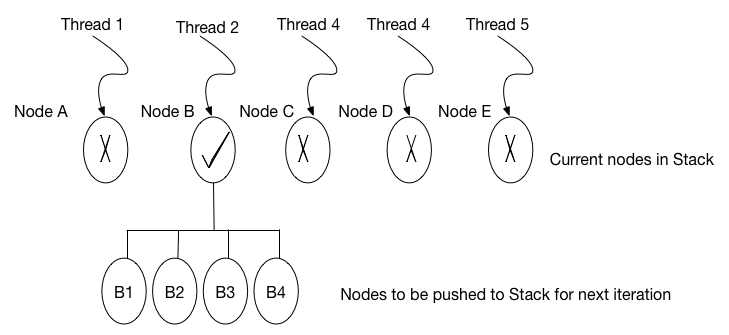
\includegraphics[scale=0.5]{BFS}
\caption{BFS implementation on a GPU}
\end{figure}

In Fig 10,  the check mark indicates that the node  satisfies the query and the tree will be further traversed from this node. The cross mark indicates either that the node does not satisfy the query or the node does not exist and the threads terminate at this point without proceeding further,

The number of stack array in the shared memory per block depends on the number of warps in a block. At the most, the iterative loop processes 32 nodes at a time by default(equal to the number of threads in a warp). 
The conditional statements are changed to avoid function return statements to prevent the traversal loop from prematurely exiting and preventing the remainder of the loop body from executing.

A polygon is checked against the node of the quadtree for 3 scenarios such as Completely overlapping , Partially overlapping  and Not overlapping.
All nodes are checked for Not overlapping conditions till leaf node is reached. If a node satisfies the condition then the tree is not traversed from this node and if the node does not satisfy the condition, then its children are placed in the stack and the traversal continues.

The number of checks for a partially overlapping node is more, and use of "if" statements decreases the performance due to control divergence. If threads within a warp take different paths, then 2 passes on the different path of the code is required to execute all threads.Since different execution paths are serialized , it leads to performance penalty.

Therefore in order to reduce conditional statements(if statements), the condition for completely overlapping node is first computed on the leaf nodes and the nodes that satisfies the condition is classified as completely overlapping nodes and nodes that does not satisfy the condition is classified as partially overlapping nodes.








\begin{figure}[ht]
 \subsection{BFS implementation in GPU-Different Scenarios of query Polygon}
 The figures below show the data points (left) and its corresponding tree representation (right). These data points will be analyzed for different polygon scenarios in the next sections.
 
  \caption{Level 1}
  \centering
  \begin{minipage}[b]{0.35\textwidth}
    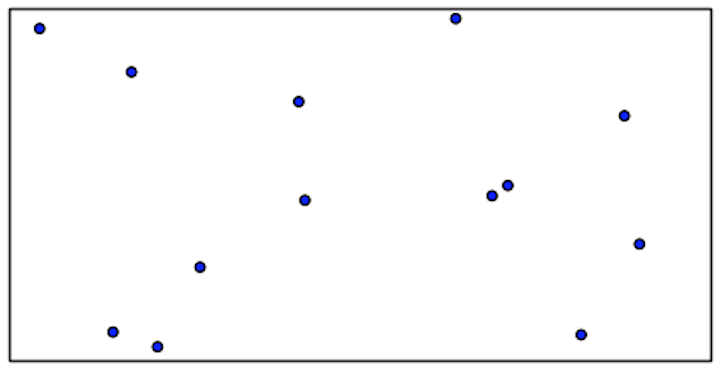
\includegraphics[width=\textwidth]{Quadtree_basic_scenario1}
  \end{minipage}
  \hfill
  \begin{minipage}[b]{0.6\textwidth}
    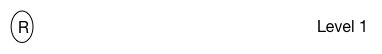
\includegraphics[width=\textwidth]{1_1Quad_1_tree}
  \end{minipage}
\end{figure}

\begin{figure}[ht]
\caption{Level 2}
  \centering
  \begin{minipage}[b]{0.35\textwidth}
    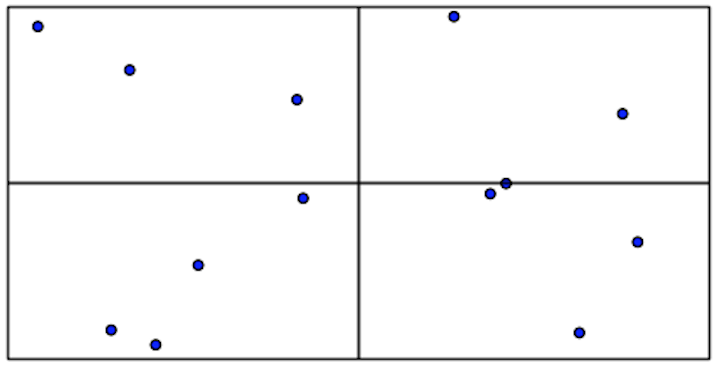
\includegraphics[width=\textwidth]{Quadtree_basic_scenario2}
  \end{minipage}
  \hfill
  \begin{minipage}[b]{0.6\textwidth}
    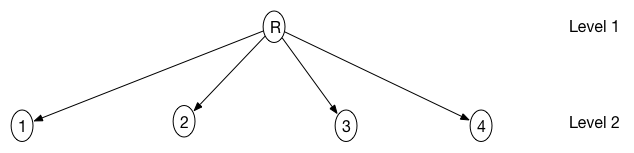
\includegraphics[width=\textwidth]{1_1Quad_2_tree}
  \end{minipage}
\end{figure}

\begin{figure}[ht]
\caption{Level 3}
  \centering
  \begin{minipage}[b]{0.35\textwidth}
    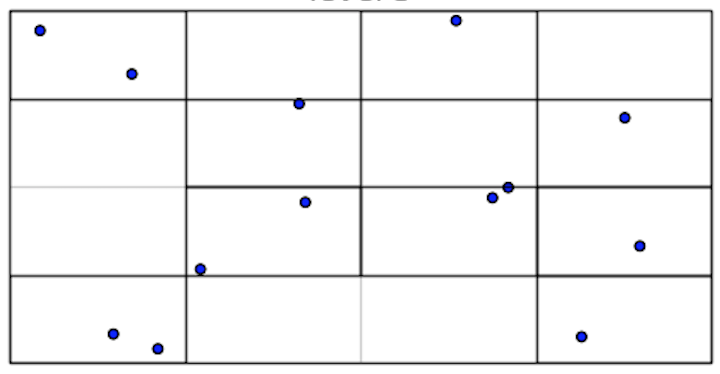
\includegraphics[width=\textwidth]{Quadtree_basic_scenario3}
  \end{minipage}
  \hfill
  \begin{minipage}[b]{0.6\textwidth}
    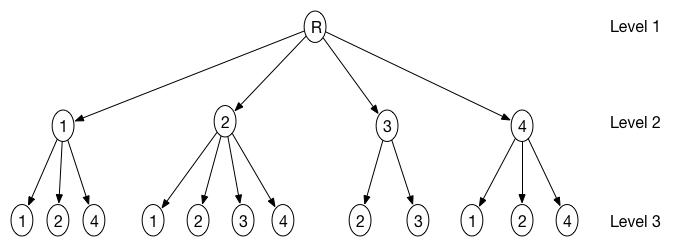
\includegraphics[width=\textwidth]{1_1Quad_3_tree}
  \end{minipage}
\end{figure}

\begin{figure}[ht]
\caption{Level 4}
  \centering
  \begin{minipage}[b]{0.35\textwidth}
    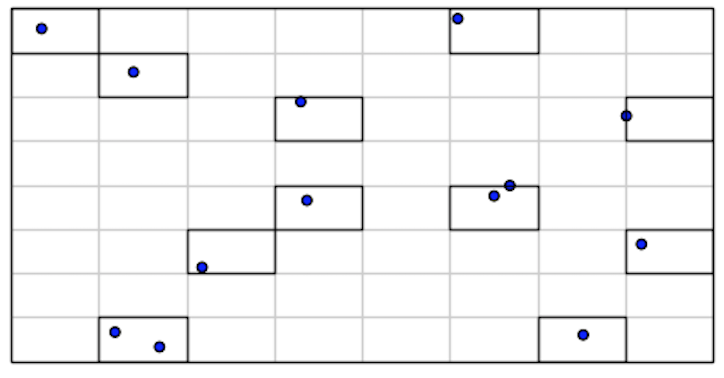
\includegraphics[width=\textwidth]{Quadtree_basic_scenario4}  
  \end{minipage}
  \hfill
  \begin{minipage}[b]{0.6\textwidth}
    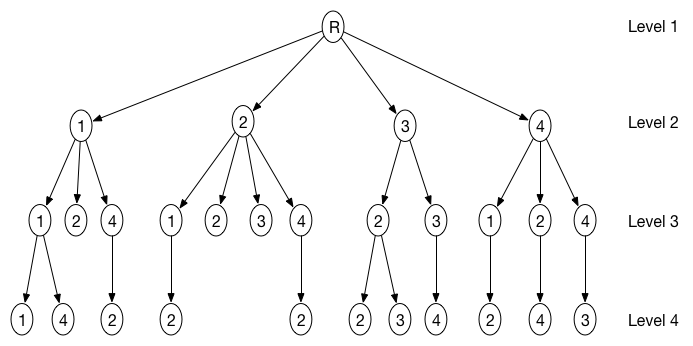
\includegraphics[width=\textwidth]{1_1Quad_4_tree}
  \end{minipage}
\end{figure}

\clearpage
\begin{figure}[ht]
\subsubsection{Query Polygon inside a leaf node}
The first scenario demonstrates the best case scenario where the polygon lies within one quadrant at level 4 of the quadtree and the algorithm provides best performance.


\caption{The figure shows the data points (left)and the quadtree(right) at Level 1.}
  \centering
  \begin{minipage}[b]{0.35\textwidth}
    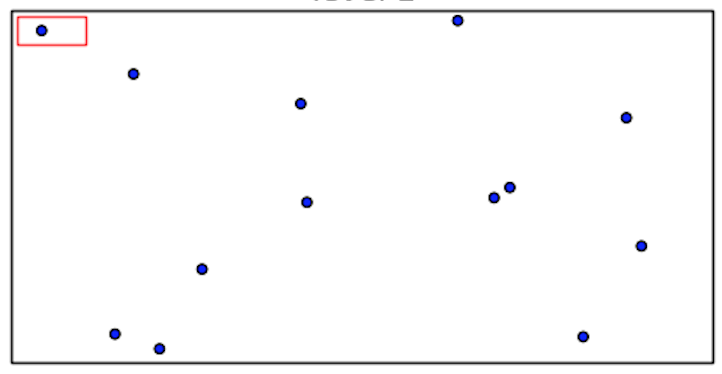
\includegraphics[width=\textwidth]{1_1Quad1_1}  
  \end{minipage}
  \hfill
  \begin{minipage}[b]{0.5\textwidth}
    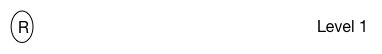
\includegraphics[width=\textwidth]{1_1Quad_1_tree}
  \end{minipage}
\end{figure}



\begin{figure}[ht]
At level 2 , the algorithm isolates  one quadrant (first child of the root node)and ignores all other quadrants, thus bringing down the number of quadrants to be processed to 1 from 4(4 is the total number of nodes at this level).
\caption{The figure below shows the data points (left)and the corresponding quadtree(right) at Level 2.}
  \centering
  \begin{minipage}[b]{0.35\textwidth}
    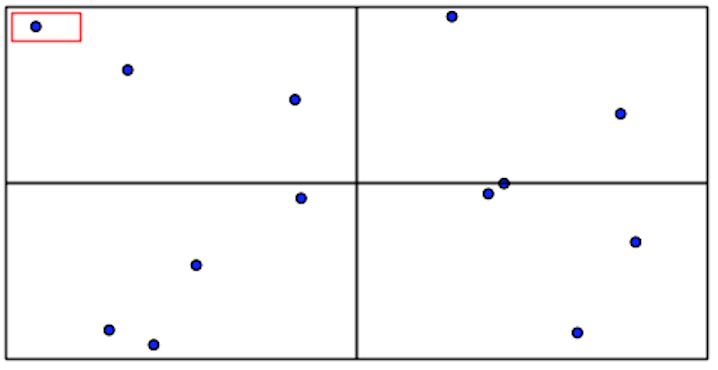
\includegraphics[width=\textwidth]{1_1Quad1_2}  
  \end{minipage}
  \hfill
  \begin{minipage}[b]{0.5\textwidth}
    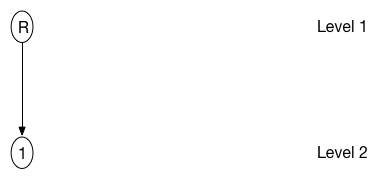
\includegraphics[width=\textwidth]{1Quad_2_tree}
  \end{minipage}
\end{figure}



\begin{figure}[ht]
At level 3, the algorithm again isolates one quadrant which is the first child of the quadrant from level 1. 
This step reduces the number of quadrants to be processed to 1 from 3(3 is the total number of children of the quadrant output from level 1).
\caption{The figure below shows the data points (left)and the corresponding quadtree(right) at Level 3.}
  \centering
  \begin{minipage}[b]{0.35\textwidth}
    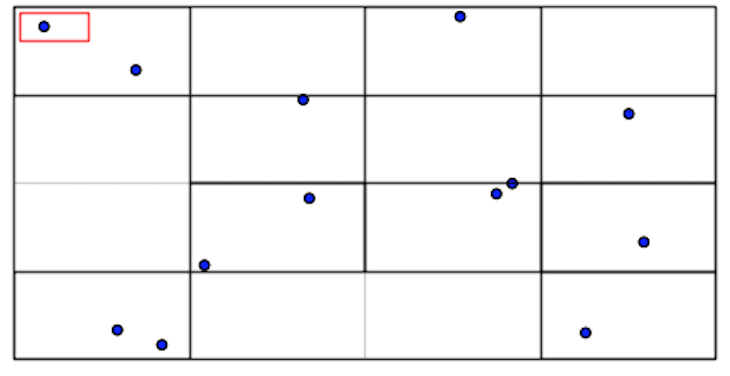
\includegraphics[width=\textwidth]{1_1Quad1_3}  
  \end{minipage}
  \hfill
  \begin{minipage}[b]{0.5\textwidth}
    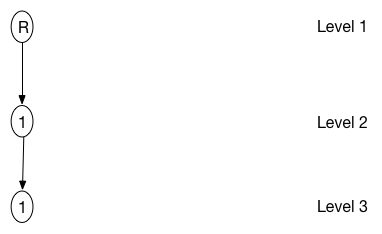
\includegraphics[width=\textwidth]{1Quad_3_tree}
  \end{minipage}
\end{figure}



\begin{figure}[ht]
At level 4, the algorithm isolates one quadrant which is the first child of the quadrant from level 3.
This step reduces the number of quadrants to be processed to 1 from 2(2 is the total number of children of the quadrant output from level 3).
Finally only one quadrant at level 4 needs to be processed in order to get the points inside the polygon in this case.
\caption{The figure below shows the data points (left)and the corresponding quadtree(right) at Level 4.}
  \centering
  \begin{minipage}[b]{0.35\textwidth}
    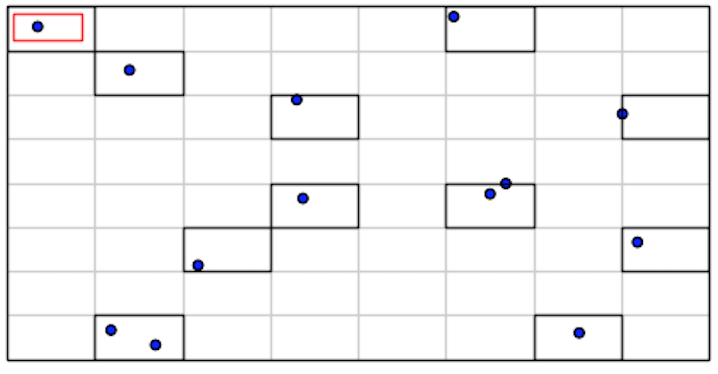
\includegraphics[width=\textwidth]{1_1Quad1_4}  
  \end{minipage}
  \hfill
  \begin{minipage}[b]{0.5\textwidth}
    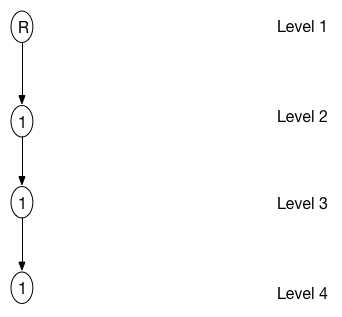
\includegraphics[width=\textwidth]{1Quad_4_tree}
  \end{minipage}
\end{figure}

\begin{figure}[ht]
\subsubsection{Polygon overlapping 2 nodes}
The second scenario demonstrates a condition where the query polygon overlaps 2 nodes at level 2 and the algorithm provides a medium performance.

\caption{The figure below shows the data points (left)and the corresponding quadtree(right) at Level 1.}
  \centering
  \begin{minipage}[b]{0.35\textwidth}
    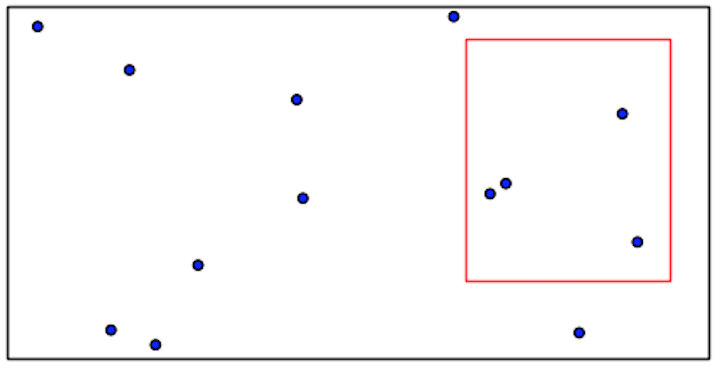
\includegraphics[width=\textwidth]{2Quad_1}  
  \end{minipage}
  \hfill
  \begin{minipage}[b]{0.6\textwidth}
    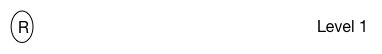
\includegraphics[width=\textwidth]{1_1Quad_1_tree}
  \end{minipage}
\end{figure}

\begin{figure}[ht]

At level 2 , the algorithm isolates  two quadrants (second and fourth child of the root node)and ignores the other two quadrants, thus bringing down the number of quadrants to be processed to 2.
\caption{The figure below shows the data points (left)and the corresponding quadtree(right) at Level 2.}
  \centering
  \begin{minipage}[b]{0.35\textwidth}
    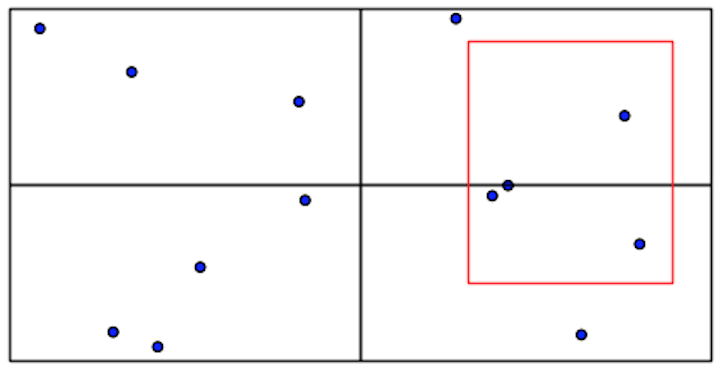
\includegraphics[width=\textwidth]{2Quad_2}  
  \end{minipage}
  \hfill
  \begin{minipage}[b]{0.6\textwidth}
    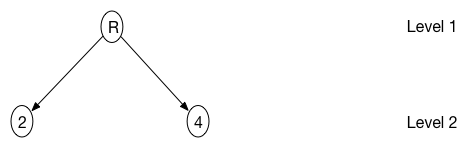
\includegraphics[width=\textwidth]{2Quad_2_tree}
  \end{minipage}
\end{figure}

\begin{figure}[ht]
At level 3, the algorithm  isolates 7 quadrants which are the all four children of the second child of root node and first and second child of the 4th child of root node.

This step does not reduce the number of nodes to be processed at this level as all the children of the nodes output from the previous level needs to be processed.
\caption{The figure below shows the data points (left)and the corresponding quadtree(right) at Level 3.}
  \centering
  \begin{minipage}[b]{0.35\textwidth}
    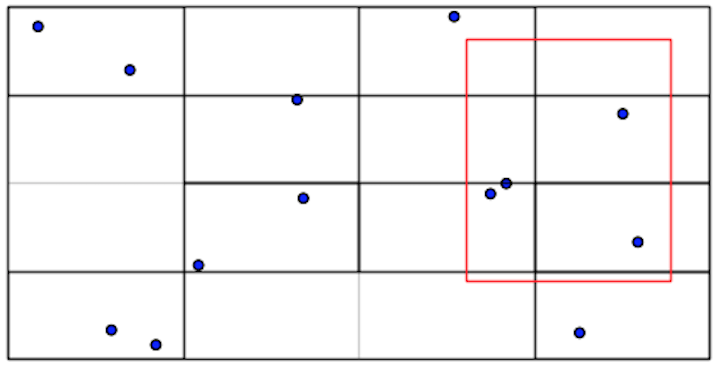
\includegraphics[width=\textwidth]{2Quad_3}  
  \end{minipage}
  \hfill
  \begin{minipage}[b]{0.6\textwidth}
    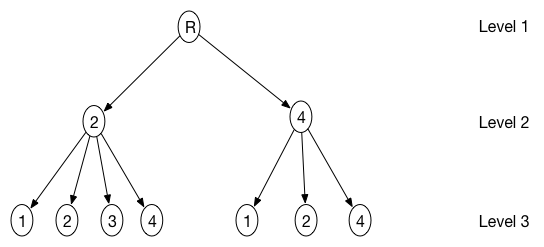
\includegraphics[width=\textwidth]{2Quad_3_tree}
  \end{minipage}
\end{figure}

\begin{figure}[ht]
At level 4, the algorithm isolates 4 quadrants from the children of 7 quadrants from previous level.By traversing down to level 4 , we are able to further reduce the number of data points that need to be evaluated by ignoring 3rd child of the 4th child from level 3.If the quadrant that is ignored at level 4 has a larger number of data points,then using a 3-level quadtree would have resulted in a huge performance penalty.

Finally only 4 quadrants at level 4 needs to be processed in order to get the points inside the polygon in this case.
\caption{The figure below shows the data points (left)and the corresponding quadtree(right) at Level 4.}
  \centering
  \begin{minipage}[b]{0.35\textwidth}
    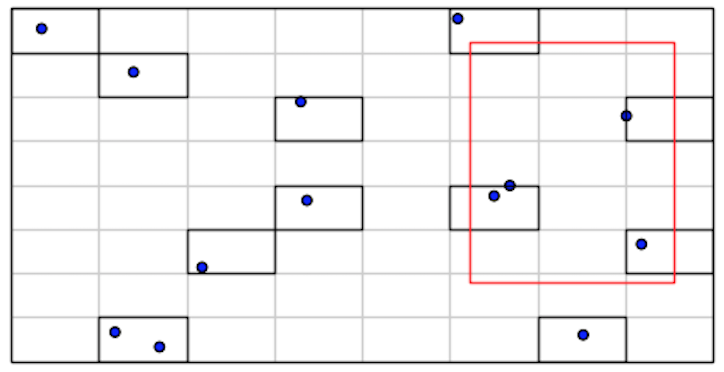
\includegraphics[width=\textwidth]{2Quad_4}  
  \end{minipage}
  \hfill
  \begin{minipage}[b]{0.6\textwidth}
    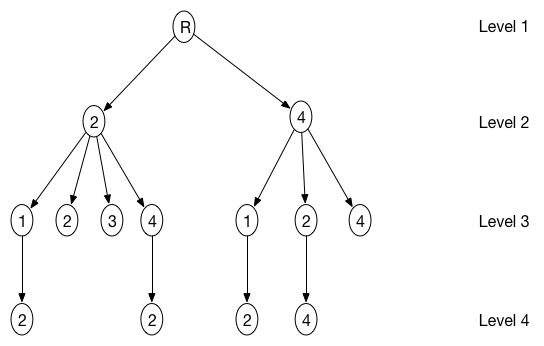
\includegraphics[width=\textwidth]{2Quad_4_tree}
  \end{minipage}
\end{figure}

\clearpage
\begin{figure}
\subsubsection{Query Polygon overlapping all leaf nodes}
The last scenario demonstrates a condition where the polygon contains maximum number of quadrants at level 4 of the quadtree and the algorithm provides a least performance compared to all other scenarios.

\caption{The figure below shows the data points (left)and the corresponding quadtree(right) at Level 2.}
  \centering
  \begin{minipage}[b]{0.35\textwidth}
    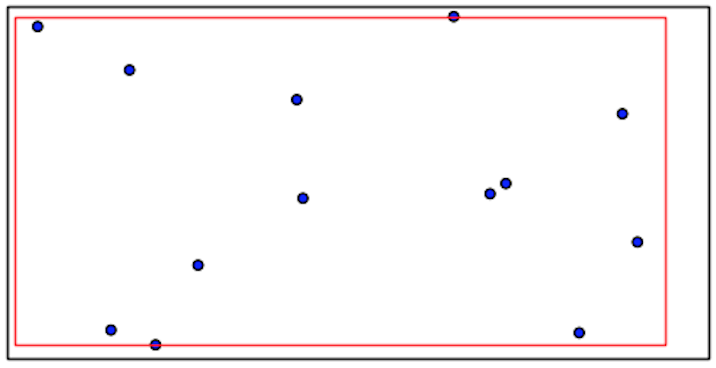
\includegraphics[width=\textwidth]{4Quad1_1}  
  \end{minipage}
  \hfill
  \begin{minipage}[b]{0.6\textwidth}
    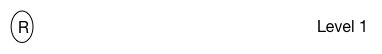
\includegraphics[width=\textwidth]{1_1Quad_1_tree}
  \end{minipage}
\end{figure}

\begin{figure}[ht]

At level 2 , the algorithm isolates all four children of the root node.
\caption{The figure below shows the data points (left)and the corresponding quadtree(right) at Level 2.}
  \centering
  \begin{minipage}[b]{0.35\textwidth}
    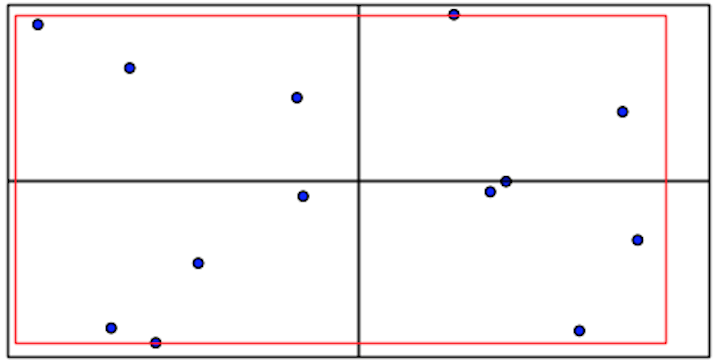
\includegraphics[width=\textwidth]{4Quad1_2}  
  \end{minipage}
  \hfill
  \begin{minipage}[b]{0.6\textwidth}
    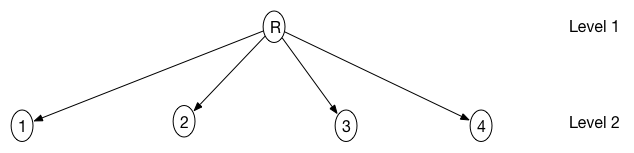
\includegraphics[width=\textwidth]{1_1Quad_2_tree}
  \end{minipage}
\end{figure}

\begin{figure}[ht]


At level 3, the algorithm  isolates all 12 quadrants at this level.The maximum possible number of nodes at this level is 16 but four of  those nodes are null nodes (it does not contain any points) and these four nodes are ignored even though these nodes lie within the polygon.
\caption{The figure below shows the data points (left)and the corresponding quadtree(right) at Level 3.}
  \centering
  \begin{minipage}[b]{0.35\textwidth}
    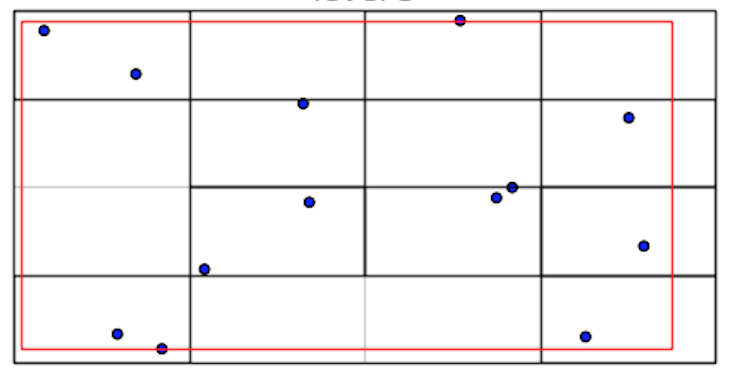
\includegraphics[width=\textwidth]{4Quad1_3}  
  \end{minipage}
  \hfill
  \begin{minipage}[b]{0.6\textwidth}
    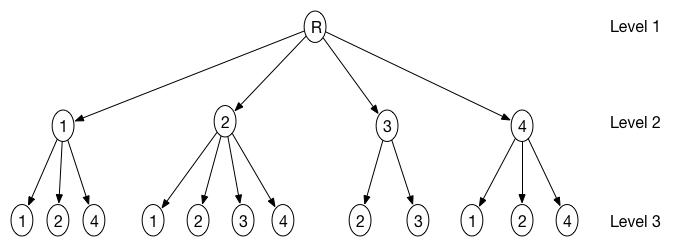
\includegraphics[width=\textwidth]{1_1Quad_3_tree}
  \end{minipage}
\end{figure}

\begin{figure}

.
At level 4, the algorithm isolates all the 11 quadrants at this level.The maximum possible number of nodes at this level is 64 but 53 of  those nodes are null nodes (it does not contain any points) and so these 53 nodes are ignored even though these nodes lie within the polygon.

Finally only 11 quadrants at level 4 needs to be processed in order to get the points inside the polygon in this case.If we assume that there are larger number of data points distributed equally across the entire 2 D space and that there are no null nodes, then all the 64 nodes need to be processed.
\caption{The figure below shows the data points (left)and the corresponding quadtree(right) at Level 4.}
  \centering
  \begin{minipage}[b]{0.35\textwidth}
    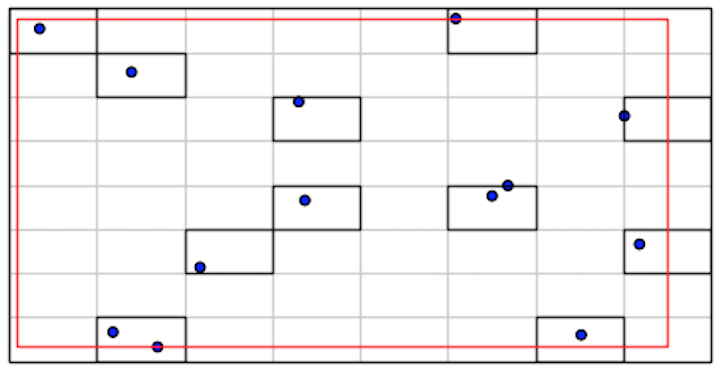
\includegraphics[width=\textwidth]{4Quad1_4}  
  \end{minipage}
  \hfill
  \begin{minipage}[b]{0.6\textwidth}
    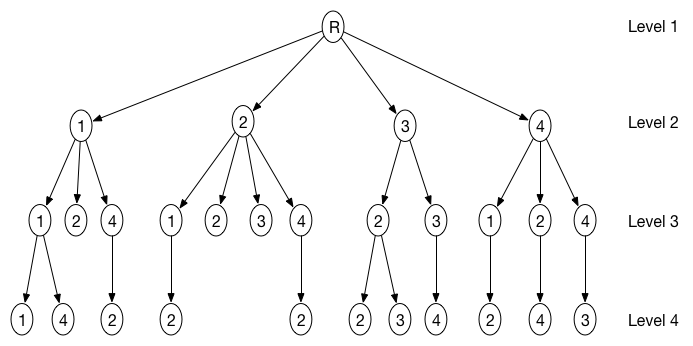
\includegraphics[width=\textwidth]{1_1Quad_4_tree}
  \end{minipage}
\end{figure}


\begin{figure}[ht]
\subsubsection{Query Polygon containing no points}

\caption{The figure below shows the data points (left)and the corresponding quadtree(right) at Level 1}
  \centering
  \begin{minipage}[b]{0.35\textwidth}
    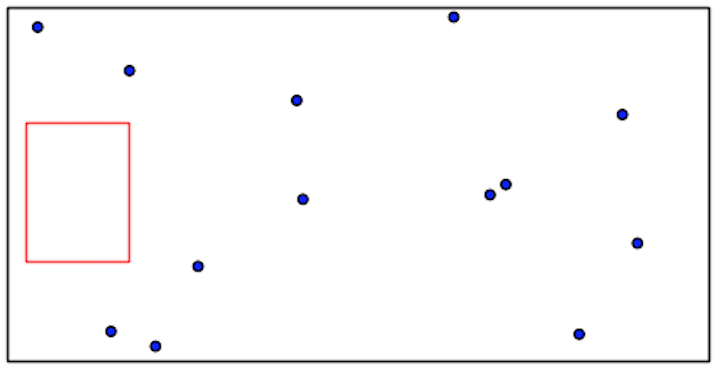
\includegraphics[width=\textwidth]{NoPointQuad1}  
  \end{minipage}
  \hfill
  \begin{minipage}[b]{0.6\textwidth}
    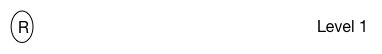
\includegraphics[width=\textwidth]{1_1Quad_1_tree}
  \end{minipage}
\end{figure}


\begin{figure}[ht]
At level 2, the algorithm isolates first and third child of the root node.

At level 3 , the polygon does not overlap with any of the children of the nodes from level 2.The nodes that it overlaps are null nodes and therefore the traversal stops at level 3.
\caption{The figure below shows the data points (left)and the corresponding quadtree(right) at Level 2}
  \centering
  \begin{minipage}[b]{0.35\textwidth}
    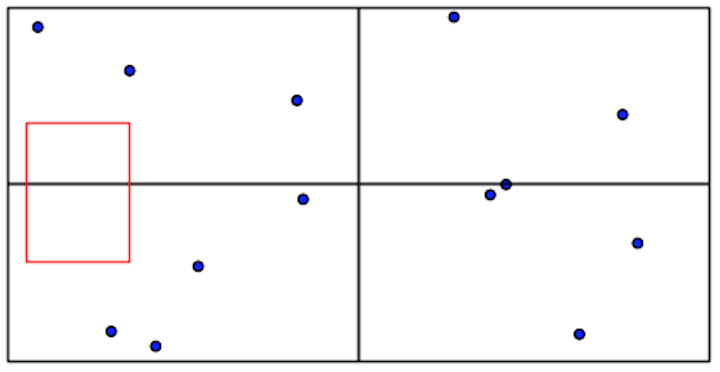
\includegraphics[width=\textwidth]{NoPointQuad2}  
  \end{minipage}
  \hfill
  \begin{minipage}[b]{0.6\textwidth}
    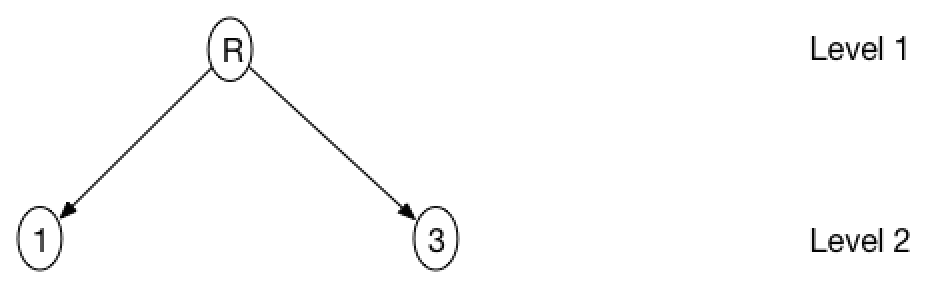
\includegraphics[width=\textwidth]{NoPoints3_1}
  \end{minipage}
\end{figure}


\clearpage
\section{Results}
The performance is compared in terms of the number polygons that can be queried per second.The number of polygons queried per second is measured for a wide range of input points. In the case of GPUs ,as the size of input increases, performance is affected due to the overhead involved in  memory transfer between CPU and GPU. But once the quadtree is transferred to the GPU, any number of polygons can be queried using iterative BFS traversal method described above. 



\begin{figure}[ht]
\caption{Performance Comparison between CPU and GPU for Small Polygons}
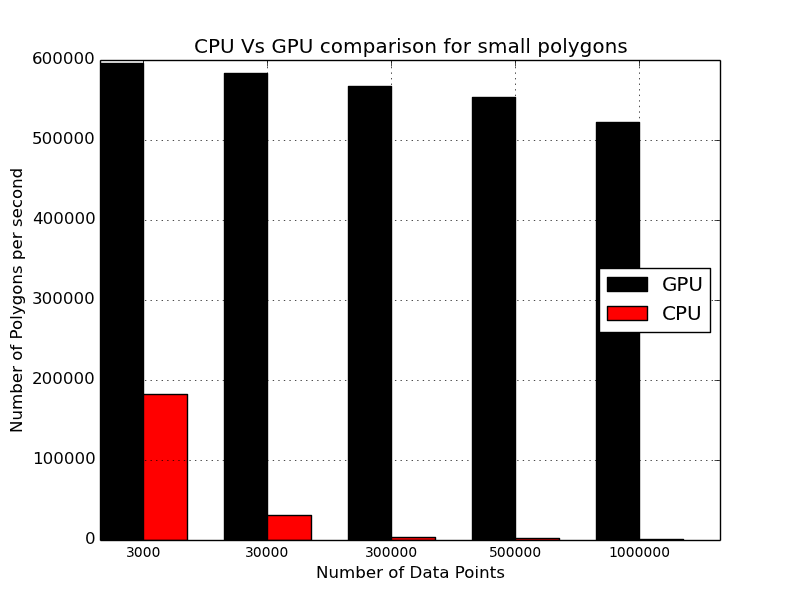
\includegraphics[scale=0.5]{CPU_GPU_SmallPoly3}

For small sized polygons the CPU-GPU approach shows a performance improvement by a factor of 3.2 for small datasets and a performance improvement by a factor of 449 for very large datasets.
\end{figure}

\begin{figure}[ht]
\caption{Performance Comparison between CPU and GPU for Medium Polygons}
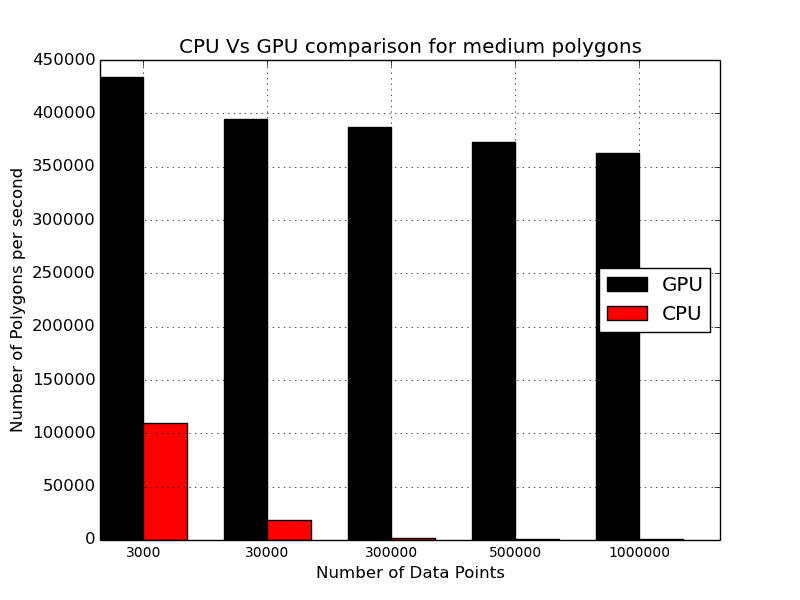
\includegraphics[scale=0.5]{CPU_GPU_MediumPoly3}

For medium sized polygons the CPU-GPU approach shows a performance improvement by a factor of 4 for small datasets and a performance improvement by a factor of 594 for very large datasets.
\end{figure}

\begin{figure}[ht]
\caption{Performance Comparison between CPU and GPU for Large Polygons}
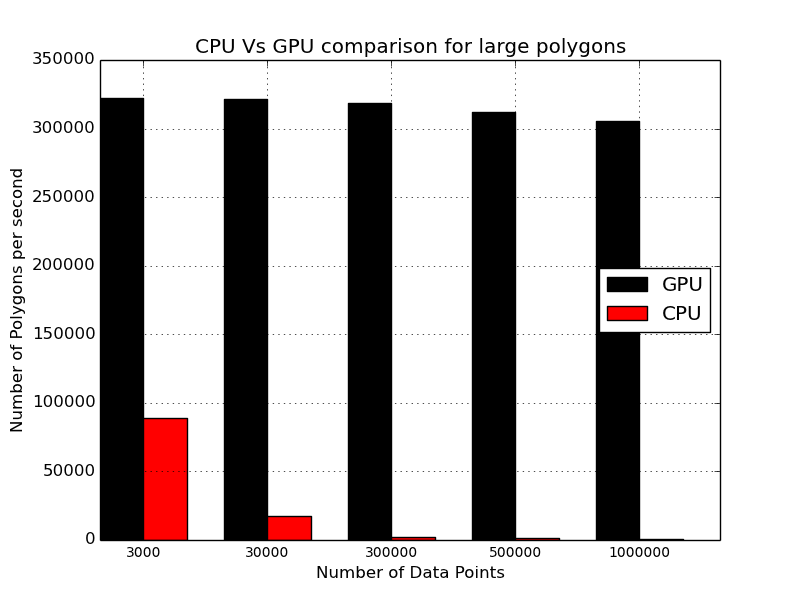
\includegraphics[scale=0.5]{CPU_GPU_LargePoly3}

For large sized polygons the CPU-GPU approach shows a performance improvement by a factor of 3.6 for small datasets and a performance improvement by a factor of 591 for very large datasets.
\end{figure}

\begin{figure}[ht]
\caption{Performance Comparison for different sized polygons using GPU}
\includegraphics[scale=0.5]{Different_Sized_Polygon_GPU4}

Similar to CPU, the GPU performs better on smaller polygons compared to the larger polygons.
In this case, the smaller polygons occupy 10 to 20 percent of the region  and the larger polygons occupy 70 to 90 percent of the region. Once the leaf nodes are reached, the number of nodes that need to be taken into account to compute points are very less  but for a large polygon which could contain a maximum of 64 nodes for a level 4 quadtree , points within all these 64 nodes need to be taken into account. 

\end{figure}


\begin{figure}[ht]
\caption{Execution time of Least to Most Complex Medium Sized Polygons}
\includegraphics[scale=0.5]{LToMCmplxMedP}

The performance is determined by the number of partial nodes a polygon contains because for partial nodes, each point inside a node needs to be checked against a polygon boundary whereas in the case of completely overlapping nodes only the range of points a node contains is stored.
The Fig 35, shows the execution time of individual medium sized polygons with a data input size of 3000.The polygons are ranked based on the number of partial nodes it contains and its execution time is measured.
The number of polygons per second calculated is the average of the output of all these individual polygons.

\end{figure}

\begin{figure}[ht]
\caption{Speed Up of GPU over CPU}
\includegraphics[scale=0.5]{SpeedUp}

The performance between CPU and GPU is measured for different sizes of polygons and the maximum performance gain is achieved for the medium polygons which are more computationally intensive than small polygons.Very less number of threads are active for small polygons  and this does not take advantage of the throughput oriented nature of the GPU.The work on medium sized polygons is optimum for the GPU as the performance decreases a little  for larger polygons.
The performance is mainly determined by the number of partial nodes a polygon contains. In the case of CPU, all the partial nodes in a polygon are processed sequentially but in the case of GPU 32 partial nodes within a polygon could processed simultaneously with a large number of polygons being queried at the same time.

\end{figure}






\end{document}















